\chapter{Experiments}
\section{Datasets}
To highlight the unique capabilities our generative approach offers, we wish to target video inpainting tasks in which visual information in nearby frames cannot be easily exploited to achieve a convincing result. The YouTube-VOS \citep{youtubevos1} (training and test) and DAVIS \citep{davis} (test) video object segmentation datasets have become the \emph{de facto} standard benchmark datasets for video inpainting in recent years, and the foreground object masks included in these datasets have led to a heavy focus on object removal tasks in qualitative evaluations of video inpainting methods. Object removal in these datasets is a task to which, for instance, optical flow-based approaches are specifically well suited, as the backgrounds are often near-stationary and so information in neighboring frames can be used to great effect. In contrast, we wish to focus on tasks where inpainting requires the visual appearances of objects to be hallucinated in whole or in part and realistically propagated through time, or where the behavior of occluded objects must be inferred. We propose four new large-scale video inpainting datasets targeting such tasks. All datasets are 256 $\times$ 256 resolution and 10 fps. Details of how each dataset was constructed, are included in \Cref{app:datasetss}.
%Additionally, the YouTube-VOS training set is problematic for training with our generative approach, as the videos are semantically diverse and the scale of the dataset is small \hlk{(3471 videos containing $\sim$200 frames each)} relative to datasets typically used to train video generative models.
\subsection{BDD-Inpainting}
We adapt the BDD100K \citep{bdd100k} dataset for the video inpainting task. This dataset contains 100,000 high-quality first-person driving videos and includes a diversity of geographic locations and weather conditions. We select a random subset of approximately 50,000 
of these, and generate a set of both moving and stationary masks of four types: grids, horizontal or vertical lines, boxes (\Cref{fig:traffic-scenes}), and blobs (\Cref{fig:fig1}). During training both videos and masks are sampled uniformly, giving a distribution over an extremely varied set of inpainting tasks. We include two test sets of 100 video-mask pairs each, the first (BDD-Inpainting) containing only grid, line, and box masks, and the second (BDD-Inpainting-Blobs) containing only blob masks. The second is a substantially more challenging test set, as the masks are often large and occlude objects in the scene for a significant period of time. See \Cref{fig:bdd-examples} for representative examples; mask types, shown in green, are indicated for each. The test sets we use, along with code for processing the original BDD100K dataset and generating masks, will be released upon publication. 
\begin{figure}
    \begin{center}
        \centering
        \captionsetup{type=figure}
        \includegraphics[width=\linewidth]{figures/dataset-examples/bdd-examples.pdf}
        \captionof{figure}{Representative examples from the BDD-Inpainting dataset.}
        \label{fig:bdd-examples}
    \end{center}
    \end{figure}
\subsection{Inpainting-Cars and Inpainting-Background}
We use an in-house dataset of overhead drone footage of vehicle traffic, for which we have tracker-generated bounding boxes for each vehicle, to create two task-specific datasets. The first, Inpainting-Background (\Cref{fig:background}), targets the removal of cars from videos by using time-shifted bounding boxes as occlusion masks, where the bounding boxes are shifted such that the masked-out region contains only the road surface and other environmental factors. The second, Inpainting-Cars (\Cref{fig:cars}), targets the \emph{addition} of cars to videos by using the original bounding boxes as masks so that the masked-out region always contains a single vehicle. Note that the masked-out vehicle is not visible at any time in the context, and so,  given an input, the model must hallucinate a vehicle and propagate it through time, using only the size and movement of the mask as clues to plausible vehicle appearance and motion. See See \Cref{fig:cars-examples} and \Cref{fig:bg-examples} for examples from the Inpainting-Cars and Inpainting-Background datasets, respectively; masks are shown in black.
\begin{figure}
    \begin{center}
        \centering
        \captionsetup{type=figure}
        \includegraphics[width=\linewidth]{figures/dataset-examples/cars-examples.pdf}
        \captionof{figure}{Representative examples from the Inpainting-Cars dataset.}
        \label{fig:cars-examples}
    \end{center}
\end{figure}
\begin{figure}
    \begin{center}
        \centering
        \captionsetup{type=figure}
        \includegraphics[width=\linewidth]{figures/dataset-examples/bg-examples.pdf}
        \captionof{figure}{Representative examples from the Inpainting-Background dataset.}
        \label{fig:bg-examples}
    \end{center}
\end{figure}
\subsection{Traffic Scenes}
Using the same in-house dataset as referenced above, we generate another dataset where large sections of the roadway are occluded, requiring the model to infer vehicle behavior in the masked-out region. Crops are centered over road features like intersections, roundabouts, highway on-ramps, \etc where complex vehicle behavior and interactions take place. This dataset contains exceptionally challenging video inpainting tasks as vehicles are often occluded for long durations of time, requiring the model to generate plausible trajectories that are semantically consistent with both the observations (e.g. the entry and exit point of a vehicle from the masked region) and the roadway. This dataset contains approximately 13,000 videos in the training set and 100 video-mask pairs in the test set. See \Cref{fig:ts-examples} for representative examples; mask types, shown in green, are indicated for each example.
\begin{figure}
    \begin{center}
        \centering
        \captionsetup{type=figure}
        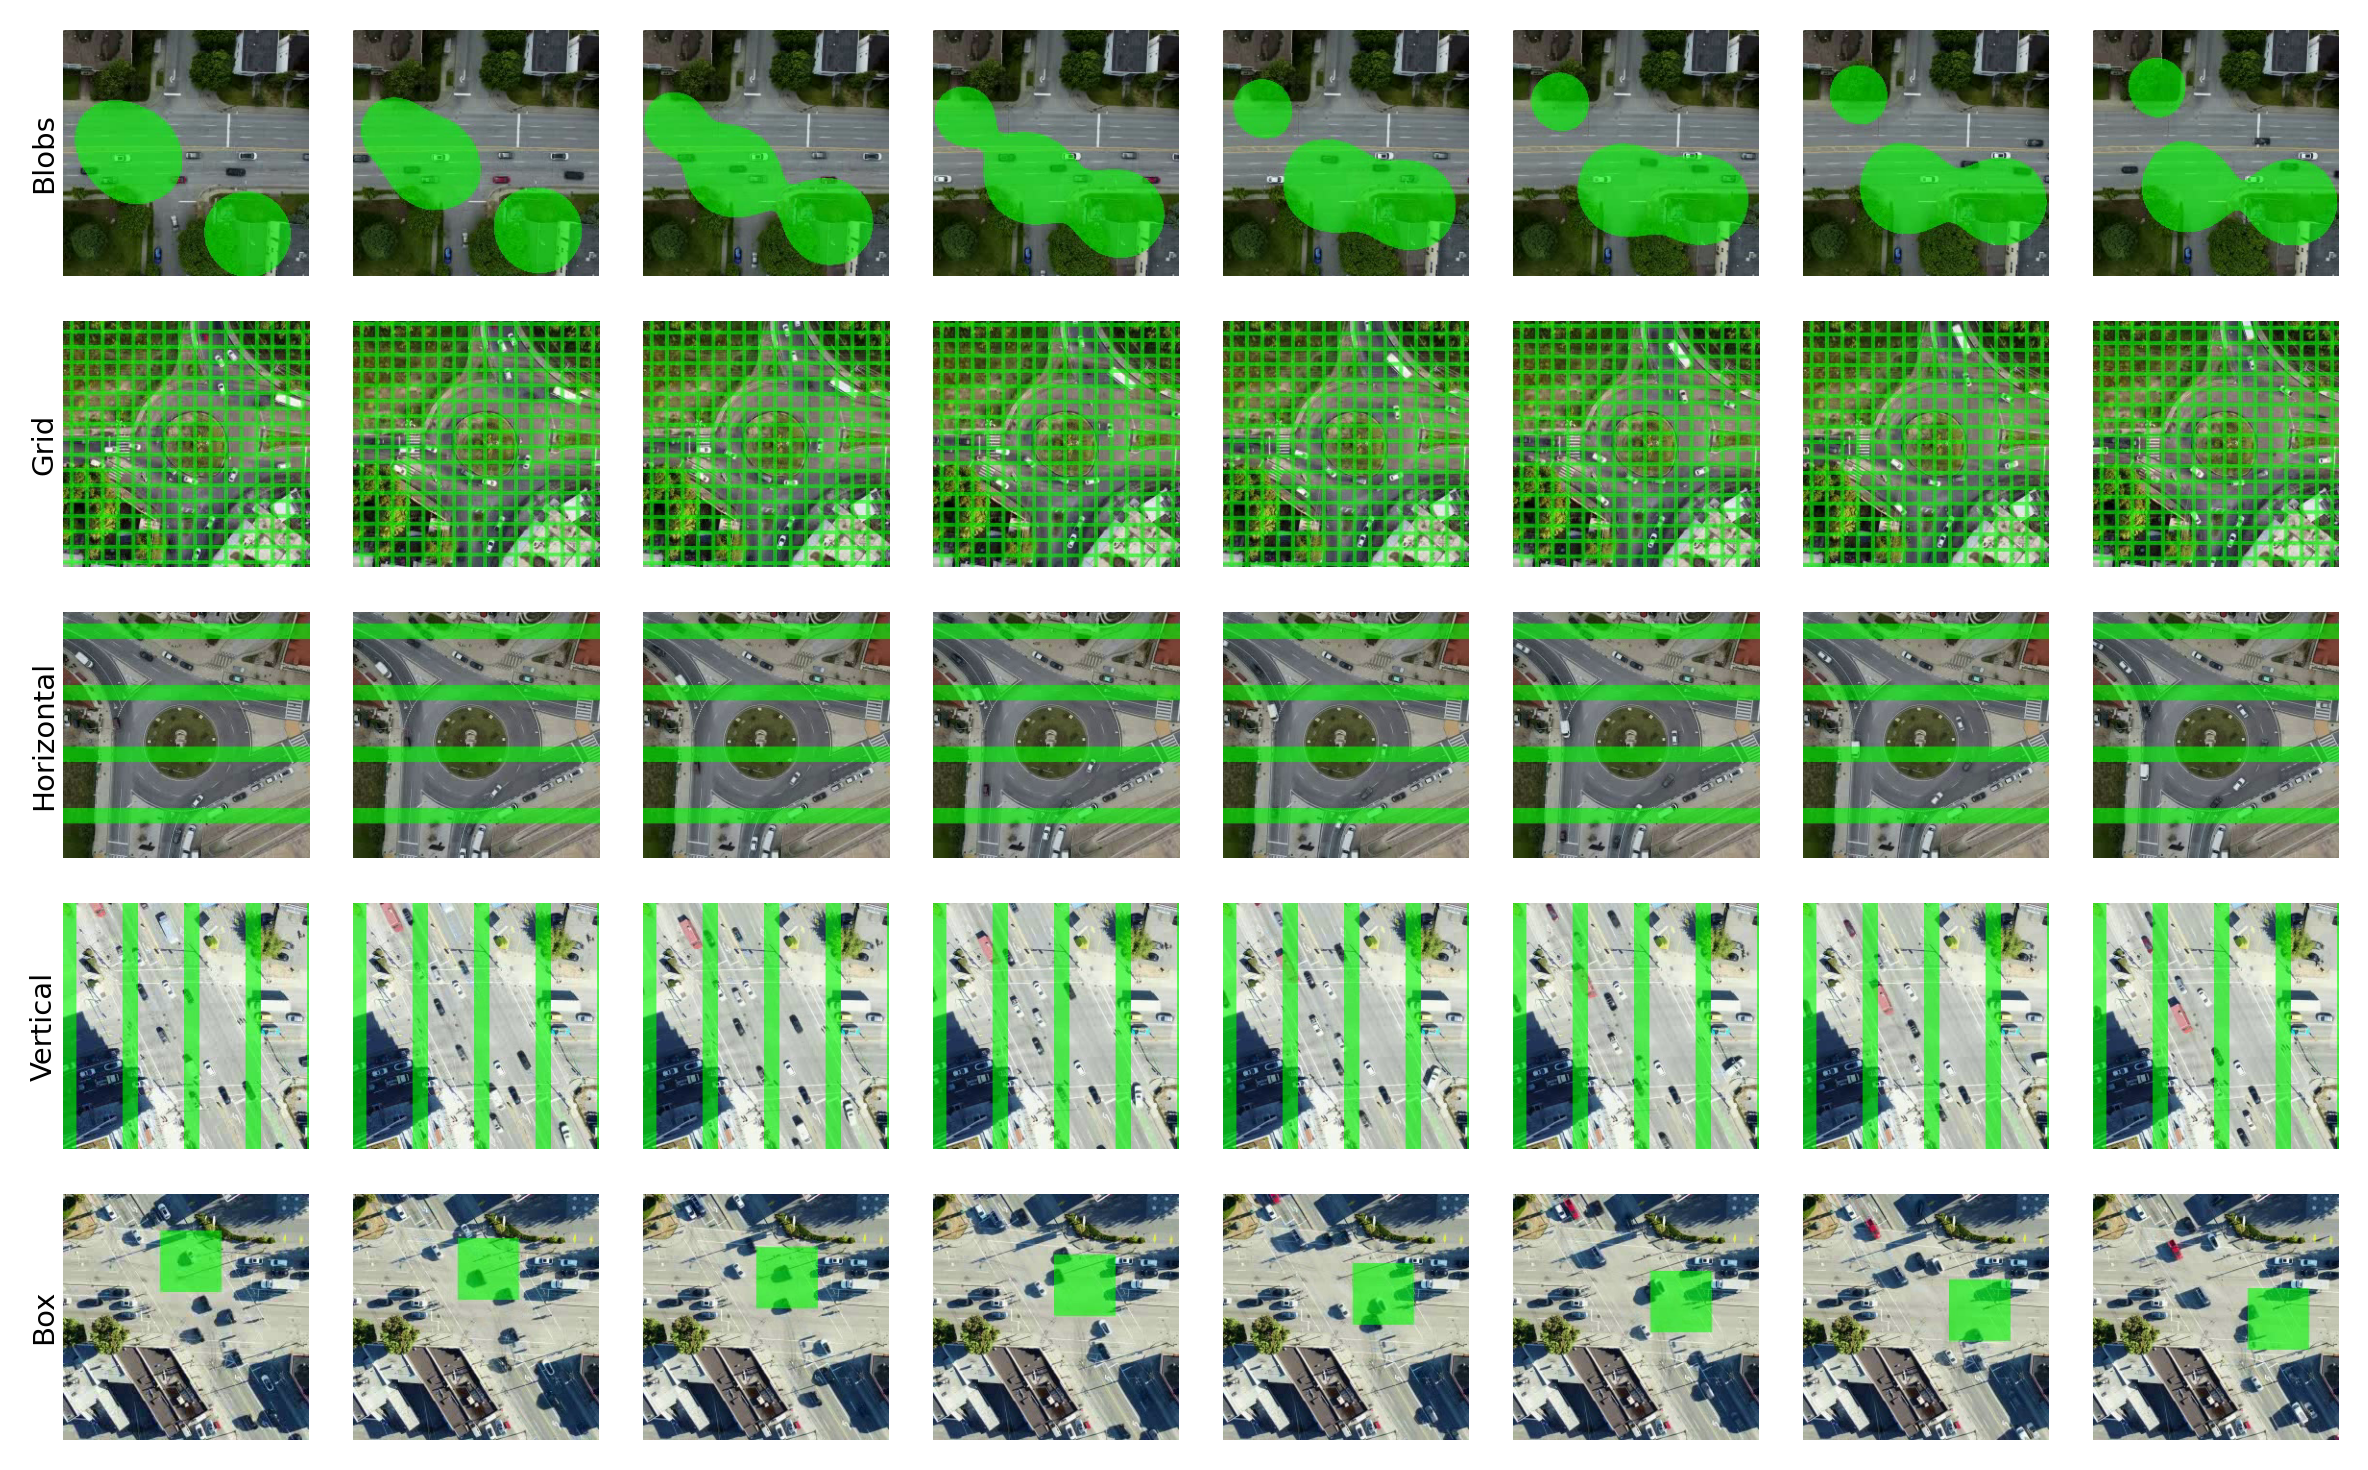
\includegraphics[width=\linewidth]{figures/dataset-examples/ts-examples.png}
        \captionof{figure}{Representative examples from the Traffic-Scenes dataset.}
        \label{fig:ts-examples}
    \end{center}
    \end{figure}

\begin{figure}
    \centering
    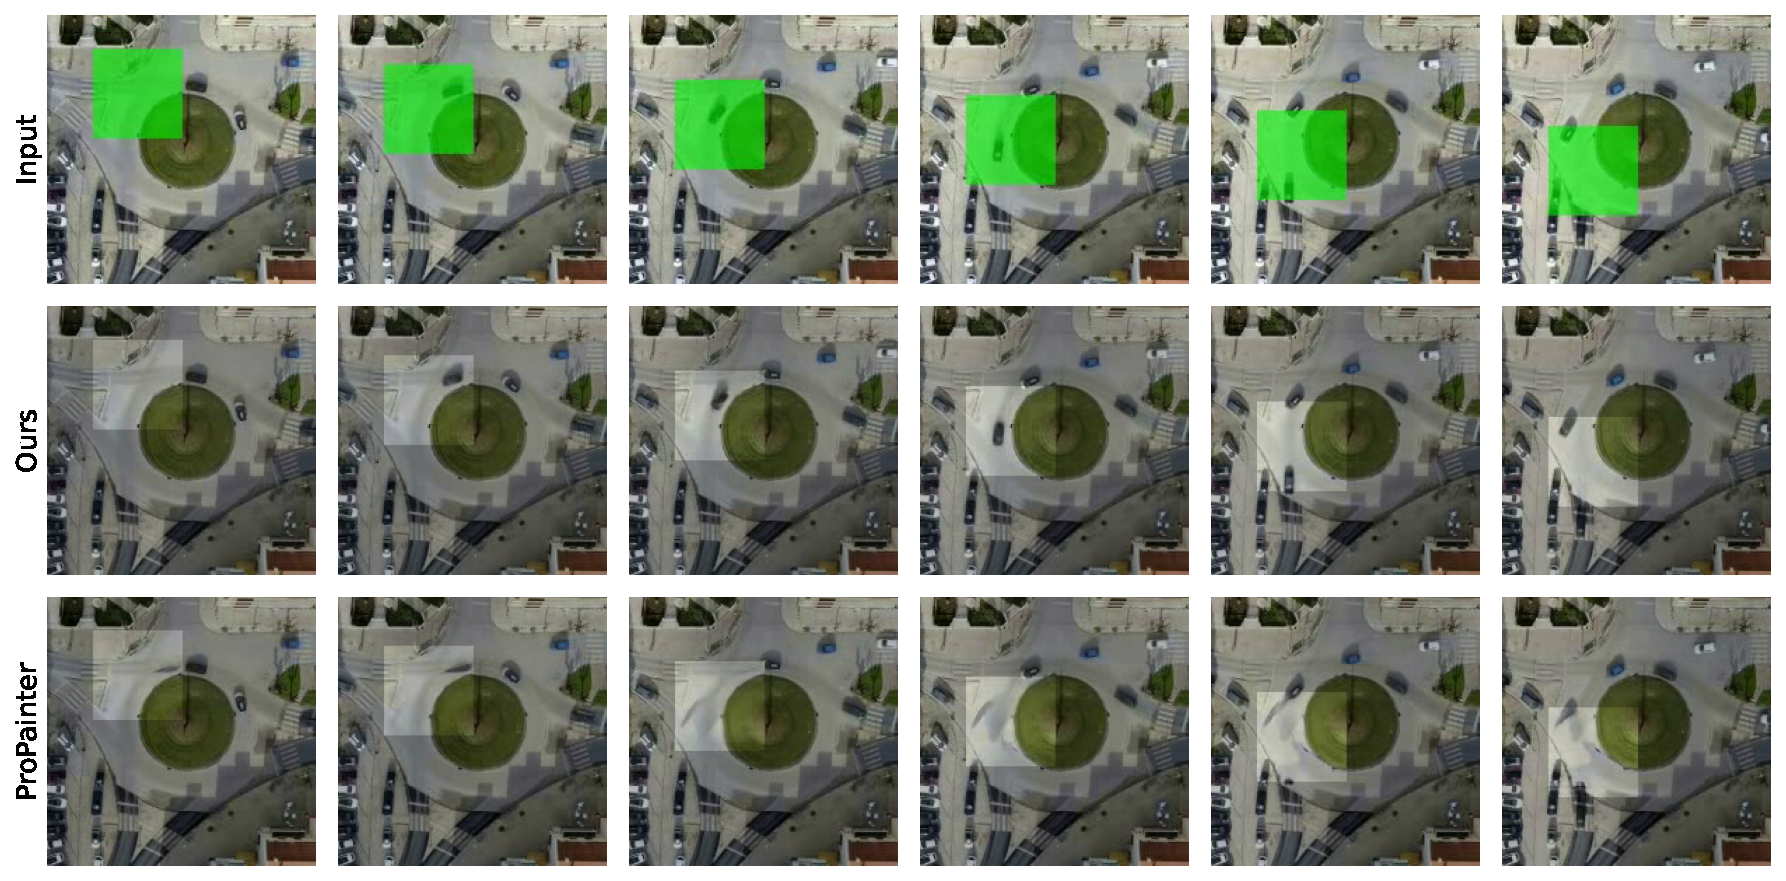
\includegraphics[width=\linewidth]{figures/13269_shaded_cropped.pdf}
    \caption[Inpaintings from our model and ProPainter on the task introduced in \Cref{fig:semantics} from our Traffic-Scenes dataset.]{Inpaintings from our model and ProPainter on the task introduced in \Cref{fig:semantics} from our Traffic-Scenes dataset. Our model can inpaint a realistic trajectory for the occluded vehicle. Competing flow-based approaches correctly inpaint the background but are unable to account for the vehicle.}
    \label{fig:traffic-scenes}
\end{figure}
\section{Baselines and Metrics} 
We compare our method with four recently proposed video inpainting methods that achieve state-of-the-art performance on standard benchmarks: ProPainter \citep{propainter}, E$^2$FGVI \citep{endtoend}, FGT \citep{fgt}, and FGVC \citep{flowedgeguided}. For each model, we use pre-trained checkpoints made available by the respective authors. We adopt the evaluation suite of DEVIL \citep{devil}, which includes a comprehensive selection of commonly used metrics targeting three different aspects of inpainting quality:
\begin{itemize}
    \item Reconstruction, or how well the method's output matches the ground truth: PSNR, SSIM \citep{ssim}, LPIPS \citep{lpips}, PVCS \citep{devil}. 
    \item Perceptual realism, or how well the appearance and/or motion resembles a reference set of ground truth videos: FID \citep{fid}, VFID \citep{vfid}.
    \item Temporal consistency: Flow warping error ($E_\text{warp}$) \citep{ewarp}, which measures how well an inpainting follows the optical flow as calculated on the ground truth. 
\end{itemize} 
For our method, we train one model on each dataset with $K=16$. Models are trained on 4$\times$ NVIDIA A100 GPUs for 1-4 weeks. A detailed accounting of each model's hyperparameters and training procedure can be found in the appendix.

\begin{figure}
    \begin{center}
        \centering
        \captionsetup{type=figure}
        \includegraphics[width=\linewidth]{figures/updated-cars.pdf}
        \caption[Inpaintings from our model on the Inpainting-Cars dataset.]{Inpaintings from our model on the Inpainting-Cars dataset. The first row is the masked input to the model, the lower two rows are two separate inpaintings sampled from our model.}
        \label{fig:cars}
    \end{center}%
\end{figure}

\begin{figure}
    \centering
    \includegraphics[width=\linewidth]{figures/bg_3119.pdf}
    \caption[A comparison of inpaintings from our method and FGT on a video from our Inpainting-Background dataset.]{Inpainted videos from our Inpainting-Background dataset. Results from our method are displayed on the top row; results from the best competing model FGT \citep{fgt} are on the bottom row. The ground truth region is darkened slightly to aid in visualizing the boundary between generated and ground-truth regions. Despite FGT outperforming our method on quantitative metrics, qualitative results are similar in quality.}
    \label{fig:background}
\end{figure}




\begin{table}[t]
\centering
\caption{Quantitative comparison with state-of-the-art video inpainting methods across each of our four datasets. For each dataset/metric, the best performing model is indicated with bold font and the second best performing model is underlined. Improved AR w/ Far Future is used for all datasets but Inpainting-Background, which uses AR.}
\label{table:main}
\customrescaleone{

\begin{tabular}{llllllll}
\toprule
Method & PSNR$\blacktriangle$ & SSIM$\blacktriangle$   & LPIPS$\blacktriangledown$     & PVCS$\blacktriangledown$   & FID$\blacktriangledown$   & VFID$\blacktriangledown$   & $E_\text{warp}$$\blacktriangledown$ \\ 
\midrule
\multicolumn{8}{c}{BDD-Inpainting} \\
\midrule
ProPainter                       & \hlk{\underline{32.65}}  & \hlk{\underline{0.968}} & \hlk{\underline{0.0355}} & \hlk{\underline{0.2806}} & \hlk{\underline{2.51}}  & \hlk{\underline{0.1599}} & \hlk{$\mathbf{\,1.5{\cdot}10^{\shortminus3}}$}            \\
FGT                              & \hlk{28.50}  & \hlk{0.928} & \hlk{0.0843} & \hlk{0.6430} & \hlk{9.94}  & \hlk{0.7863} & \hlk{$\,4.0{\cdot}10^{\shortminus3}$}          \\
E$^2$FGVI                        & \hlk{30.16}  & \hlk{0.946} & \hlk{0.0640} & \hlk{0.4765} & \hlk{6.58}  & \hlk{0.3665} & \hlk{$\,2.3{\cdot}10^{\shortminus3}$}            \\
FGVC                             & \hlk{25.84}  & \hlk{0.884} & \hlk{0.1498} & \hlk{1.0210} & \hlk{32.08} & \hlk{1.7995} & \hlk{$\,7.5{\cdot}10^{\shortminus3}$}     \\
Ours                             & \hlbf{33.68}	& \hlbf{0.972} & \hlbf{0.0261} & \hlbf{0.2037}	& \hlbf{1.71}  & \hlbf{0.0748} & \hlk{\,$\underline{1.8{\cdot}10^{\shortminus3}}$} \\
\midrule
\multicolumn{8}{c}{BDD-Inpainting-Blobs} \\
\midrule
ProPainter                       & \hlk{\underline{30.54}}  & \hlk{\underline{0.960}} & \hlk{\underline{0.0467}} & \hlk{\underline{0.3120}} & \hlk{\underline{2.56}}  & \hlk{\underline{0.1499}} & \hlk{$\mathbf{\,1.2{\cdot}10^{\shortminus3}}$}               \\
FGT                              & \hlk{27.33}  & \hlk{0.938} & \hlk{0.0737} & \hlk{0.5130} & \hlk{9.41}  & \hlk{0.3594} & \hlk{$\,2.5{\cdot}10^{\shortminus3}$}            \\
E$^2$FGVI                        & \hlk{29.04}  & \hlk{0.950} & \hlk{0.0667} & \hlk{0.4414} & \hlk{4.23}  & \hlk{0.2339} & \hlk{$\,1.7{\cdot}10^{\shortminus3}$}            \\
FGVC                             & \hlk{25.10}  & \hlk{0.913} & \hlk{0.0980} & \hlk{0.6957} & \hlk{16.64} & \hlk{0.6184} & \hlk{$\,3.8{\cdot}10^{\shortminus3}$}            \\
Ours                       & \hlbf{30.67}	& \hlbf{0.961} & \hlbf{0.0442} & \hlbf{0.2857}	& \hlbf{1.69}  & \hlbf{0.1083} & \hlk{$\,\underline{1.5{\cdot}10^{\shortminus3}}$}            \\
\midrule
\multicolumn{8}{c}{Inpainting-Background} \\
\midrule
ProPainter                   & \hlk{42.03}  & \hlk{\underline{0.994}} & \hlk{0.0145} & \hlk{0.0572} & \hlk{2.83}  & \hlk{\underline{0.0550}} & \hlk{$\mathbf{\,2.6{\cdot}10^{\shortminus4}}$}            \\
FGT                          & \hlbf{44.23}  & \hlbf{0.996} & \hlbf{0.0081} & \hlbf{0.0371} & \hlbf{1.35}  & \hlbf{0.0462} & \hlk{$\,\underline{2.9{\cdot}10^{\shortminus4}}$}            \\
E$^2$FGVI                    & \hlk{37.27}  & \hlk{0.985} & \hlk{0.0400} & \hlk{0.2074} & \hlk{6.71}  & \hlk{0.2600} & \hlk{$\,6.0{\cdot}10^{\shortminus4}$}            \\
FGVC                         & \hlk{\underline{42.92}}  & \hlk{0.993} & \hlk{\underline{0.0117}} & \hlk{\underline{0.0557}} & \hlk{\underline{1.99}}  & \hlk{0.0742} & \hlk{$\,4.7{\cdot}10^{\shortminus4}$}            \\
Ours                       & \hlk{38.99}	& \hlk{0.987} & \hlk{0.0273} & \hlk{0.1443}	& \hlk{6.11}  & \hlk{0.1455} & \hlk{$\,4.1{\cdot}10^{\shortminus4}$} \\
\midrule
\multicolumn{8}{c}{Traffic-Scenes} \\
\midrule
ProPainter                   & \hlk{\underline{31.98}}  & \hlk{\underline{0.967}} & \hlk{\underline{0.0326}} & \hlk{\underline{0.2909}} & \hlk{\underline{8.51}}  & \hlk{\underline{0.3482}} & \hlk{$\,\underline{2.5{\cdot}10^{\shortminus4}}$}            \\
FGT                          & \hlk{31.97}  & \hlk{0.963} & \hlk{0.0397} & \hlk{0.3528} & \hlk{9.92}  & \hlk{0.5392} & \hlk{$\,3.6{\cdot}10^{\shortminus4}$}            \\
E$^2$FGVI                    & \hlk{31.40}  & \hlk{0.957} & \hlk{0.0440} & \hlk{0.3809} & \hlk{13.13} & \hlk{0.6113} & \hlk{$\,4.1{\cdot}10^{\shortminus4}$}            \\
FGVC                         & \hlk{29.11}  & \hlk{0.926} & \hlk{0.0794} & \hlk{0.5914} & \hlk{25.93} & \hlk{1.2358} & \hlk{$\,9.9{\cdot}10^{\shortminus4}$}            \\
Ours                         & \hlbf{35.29}	& \hlbf{0.978} & \hlbf{0.0202} & \hlbf{0.1725}	& \hlbf{4.87}  & \hlbf{0.1637} & \hlk{$\mathbf{\,2.3{\cdot}10^{\shortminus4}}$}            \\
\bottomrule
\end{tabular}}
\end{table}

\section{Quantitative Evaluation}
We report quantitative results across four of our datasets in \Cref{table:main}. For each dataset, we report metrics for the best-performing model and sampling scheme we found for that dataset. For all metrics other than $E_\text{warp}$ our method outperforms the baselines on three out of four datasets, often by a significant margin. We suspect the discrepancy between $E_\text{warp}$ and the other metrics is because each of the competing methods predicts a completion of the optical flow field and utilizes this during the inpainting process, in a sense explicitly targeting $E_\text{warp}$. On the Infilling-Background dataset the baseline methods dominate, likely owing to this being precisely the kind of task that flow-based propagation is well-suited to; the (approximate) ground truth is visible in neighbouring frames. Infilling-Cars is omitted from this section, as we are not aware of an existing method suitable for this task. 


\section{Qualitative Evaluation}
\subsection{BDD-Inpainting}
On this dataset, qualitative differences between our method and competing approaches are most evident in the presence of large masks that partially or fully occlude objects for a long period of time or the entire video. In such cases our method can retain or complete the visual appearance of occluded objects and propagate them through time in a realistic way, while such objects tend to disappear gradually with flow-based approaches (as in \Cref{fig:fig1}). Qualitative results on this dataset are heavily influenced by the sampling scheme used. As demonstrated in \Cref{sec:samplingschemes}, our ``Improved AR w/ Far Future'' sampling scheme tends to perform best, as it allows us to incorporate information from both past and future frames in the inpainting process. \Cref{fig:bus} and \Cref{fig:taxi} show additional results on tasks from the BDD-Inpainting test set.
\begin{figure}
\begin{center}
    \centering
    \captionsetup{type=figure}
    \includegraphics[width=\linewidth]{figures/additional-samples/bus_all.pdf}
    \caption[Qualitative results from our method and all competing methods on an example from the BDD-Inpainting-Blobs test set.]{Qualitative results from our method and all the competing methods we compared to quantitatively on an example from the BDD-Inpainting test set. We note that, in the presence of small masks, the qualitative differences are less pronounced between our method and the best-performing benchmarks, like since information in neighbouring frames can more easily be exploited. For our method we use the Improved AR w/ Far Future sampling scheme.}
    \label{fig:bus}
\end{center}
\end{figure}
    
    
    
\begin{figure}
\begin{center}
    \centering
    \captionsetup{type=figure}
    \includegraphics[width=\linewidth]{figures/additional-samples/taxi_all.pdf}
    \caption[Qualitative results from our method and all competing methods on an example from the BDD-Inpainting test set.]{Qualitative results from our method and all the competing methods we compared to quantitatively on an example from the BDD-Inpainting test set. Again, for our method we use the Improved AR w/ Far Future sampling scheme. In this video the vehicle passing in the left-hand lane is only ever partially visible, causing other methods to produce blurry results. }
    \label{fig:taxi}
\end{center}
\end{figure}

\subsection{Traffic-Scenes} On this dataset, all competing methods tend to inpaint only the road surface; when vehicles enter the occluded region they disappear almost instantaneously. Our method shows a surprising ability to inpaint long, realistic trajectories that are consistent with the entry/exit points of vehicles into the occluded region, as well as correctly following roadways as in \Cref{fig:traffic-scenes}. \Cref{fig:ts1} and \Cref{fig:ts2} show additional results on tasks from the Traffic-Scenes test set.%Despite this, the vehicles themselves often lack temporal consistency, changing appearance during the time they are occluded. We also often have vehicles that disappear, likely caused by cases where \eg the exit point is not observed until late into the occlusion period and the partially inpainted trajectory is inconsistent with it. 
\begin{figure}
\begin{center}
    \centering
    \captionsetup{type=figure}
    \includegraphics[width=\linewidth]{figures/additional-samples/ts1.pdf}
    \caption[Qualitative results from our method and all competing methods on an example from the Traffic-Scenes test set.]{Qualitative results from our method and all the competing methods we compared to quantitatively on an example from the Traffic-Scenes test set. For our method we use the Hierarchy-2 sampling scheme. For our method the two occluded vehicles are inpainted with continuous trajectories; for all other methods the vehicles disappear while they are occluded.} 
    \label{fig:ts1}
\end{center}
\end{figure}
    
\begin{figure}
\begin{center}
    \centering
    \captionsetup{type=figure}
    \includegraphics[width=\linewidth]{figures/additional-samples/ts2.pdf}
    \caption[Further qualitative results from our method and all competing methods on another example from the Traffic-Scenes test set.]{Further qualitative results from our method and all the competing methods we compared to quantitatively on an example from the Traffic-Scenes test set. In the ground truth for this example, in the first frame there is a vehicle making a left hand turn towards the bottom of the image that is occluded until it briefly emerges many frames later. Our model is able to initialize a vehicle in the inpainting and complete a trajectory which is consistent with the exit point for the vehicle. In all other methods the vehicle appears suddenly. } 
    \label{fig:ts2}
\end{center}
\end{figure}
\subsection{Inpainting-Background}
Qualitatively, all methods perform similarly on this dataset. Specifically, regardless of which method is used, it is difficult to tell where the masked region is without a visual aid on most inpainted videos (see \Cref{fig:background}). In some examples where the ground stays stationary for an extended period of time, our method produces artifacts that are likely to contribute to its poor performance on this dataset
compared to the others. 

\subsection{Inpainting-Cars}
Sampled inpaintings from our model on an example from the Inpainting-Cars dataset are shown in \Cref{fig:cars} and \Cref{fig:extra-cars}. Our model is capable of generating diverse, visually realistic inpaintings for a given input. We note the model's ability to use \emph{semantic} cues from the context to generate plausible visual features, such as realistic behavior of shadows and plausible turning trajectories based only on the movement of the mask.

\begin{figure}
    \centering
    \begin{subfigure}{\textwidth}
        \centering
        \includegraphics[width=\textwidth]{figures/additional-samples/cars_3028.pdf}
        \label{fig:extra-cars1}
    \end{subfigure}
    ~
    \begin{subfigure}{\textwidth}
        \centering
        \includegraphics[width=\textwidth]{figures/additional-samples/cars_3067.pdf}
        \label{fig:extra-cars2}
    \end{subfigure}
    ~
    \begin{subfigure}{\textwidth}
        \centering
        \includegraphics[width=\textwidth]{figures/additional-samples/cars_3093.pdf}
        \label{fig:extra-cars3}
    \end{subfigure}%
    \caption[Additional qualitative results from our method on the Inpainting-Cars
    test set.]{Additional qualitative results from our method on the Inpainting-Cars test set, demonstrating our method's ability to generate diverse vehicle appearances to inpaint the scene and to deal with various complications in the context.  In \Cref{fig:extra-cars1}, our method is able to deal with partial occlusion by trees in the scene. In \Cref{fig:extra-cars2}, note that the inpainted cars' shadows are oriented in the same direction as the shadows of other objects. \Cref{fig:extra-cars3} demonstrates that our method is capable of realistically shading an inpainted vehicle's color when it enters the shade.
    }
    \label{fig:extra-cars}
\end{figure}

\section{Ablations}

\subsection{Effect of Sampling Schemes}
We compare selected sampling schemes on the Traffic-Scenes dataset in \Cref{table:samplingschemes}, before providing more thorough qualitative and quantitative comparisons in the appendix. Improved AR w/ Far Future is the best on all datasets aside from Infilling-Background in terms of video realism (VFID) and temporal consistency (warp error), demonstrating the importance of our method's ability to condition on incomplete frames. AR tends to do poorly on all metrics on both the Traffic-Scenes and BDD-Inpainting datasets. This is likely due to its inability to account for observed pixel values in frames coming after the ones being generated at each stage, causing divergence from the ground-truth and then artifacts when producing later frames conditioned on incompatible values. Hierarchy-2 does well on some metrics of reconstruction and frame-wise perceptual quality. It does less well in terms of video realism, as the inpainting of the ``keyframes'' in the first stage is done without conditioning on the known pixels of frames in their immediate vicinity, potentially leading to incompatibility with the local context.

To highlight the qualitative impact that different sampling schemes can have on the quality of inpainted videos, we select a video from the BDD-Inpainting test set where conditioning on the appropriate frames is crucial for our method to succeed. \Cref{fig:qual-begin} shows the beginning of this video, where a car is occluded in the right-hand lane for the first few seconds of the video (see input frames in the first row). The Autoregressive (AR) scheme (second row) shows a distinct ``pop-in'' effect, as when the initial frames were generated the model was not able to condition on future frames where the cars existence and appearance are revealed. Both Reverse-AR and AR w/ Far Future (third and fourth rows) do condition on future frames that contain the car; Reverse-AR because the model is able to propagate the car backwards through time, and AR w/ Far Future because the model conditions on frames far out into the future where the car has been revealed. \Cref{fig:qual-end} shows the end of the video, where the cars in the right-hand lane are occluded and remain occluded for the rest of the video (first row). The AR scheme keeps these cars visible, as it is able to propagate them forward through time (second row). Reverse-Autoreg (third row) fails for the same reason that Autoreg did at the beginning: when the final frames were generated, the model was not able to condition on frames where the vehicles were visible. AR w/ Far Future (fourth row) is again successful; despite the cars not becoming visble again (and thus there is no ``future'' to condition on), it is able to propagate the cars forward in time as the Autoreg scheme does. 



\begin{table}
\centering
\caption{Effect of sampling schemes, measured on the Traffic-Scenes test set.}
\label{table:samplingschemes}
\customrescaleone{
\begin{tabular}{llllllllllllll}
\toprule
Sampling Scheme & PSNR$\blacktriangle$ & SSIM$\blacktriangle$   & LPIPS$\blacktriangledown$     & PVCS$\blacktriangledown$   & FID$\blacktriangledown$   & VFID$\blacktriangledown$   & $E_\text{warp}$$\blacktriangledown$ \\ 
\midrule
AR                 & 31.72 & 0.9595 & 0.0392 & 0.2989 & 8.85 & 0.3016 & $3.01{\cdot}10^{\shortminus4}$ \\
Hierarchy-2                    & \textbf{35.53} & \textbf{0.9794} & \textbf{0.0196} & 0.1732 & \textbf{4.55} & 0.1714 & $2.48{\cdot}10^{\shortminus4}$ \\
Improved AR w/ Far Future                 & 35.29 & 0.9783 & 0.0202 & \textbf{0.1725} & 4.87 & \textbf{0.1637} & $\mathbf{2.26{\cdot}10^{\shortminus4}}$ \\
3-Res. Improved AR & 35.32 & 0.9785 & 0.0210 & 0.1815 & 5.07 & 0.1821 & $2.43{\cdot}10^{\shortminus4}$ \\
\bottomrule
\end{tabular}}
\end{table}

\subsection{Samplers and Number of Sampling Steps}
The use of diffusion models allows for a trade-off of computation time \vs inpainting quality through the number of steps used in the generative process. In \Cref{table:samplingsteps} we report the results of our model on the BDD-Inpainting test set with the AR sampling scheme using different samplers and numbers of sampling steps. Aligning with expectations and qualitative observations, performance on metrics degrades as the number of sampling steps decreases for LPIPS, PVCS, FID and VFID. We note, however, that performance on $E_\text{warp}$, PSNR, and SSIM improves, suggesting that these metrics may not correlate well with perceived quality, as has been previously suggested for the latter two metrics in \citet{perceptual}.

\begin{figure}
    \begin{center}
        \centering
        \captionsetup{type=figure}
        \includegraphics[width=\linewidth]{figures/james_quall/james_quall_beginning.pdf}
        \caption{Qualitative results from different sampling schemes on the beginning of the video discussed in \Cref{sec:samplingschemes}}
        \label{fig:qual-begin}
        \includegraphics[width=\linewidth]{figures/james_quall/james_quall_end.pdf}
        \caption{Qualitative results from different sampling schemes on the end of the video discussed in \Cref{sec:samplingschemes}}
        \label{fig:qual-end}
    \end{center}
\end{figure}

\begin{table}
\centering
\caption{Effect of diffusion samplers, using AR sampling on BDD-Inpainting.}
\label{table:samplingsteps}
\customrescaleone{
\begin{tabular}{llllllllllllll}
\toprule
Sampler & PSNR$\blacktriangle$ & SSIM$\blacktriangle$   & LPIPS$\blacktriangledown$     & PVCS$\blacktriangledown$   & FID$\blacktriangledown$   & VFID$\blacktriangledown$   & $E_\text{warp}$$\blacktriangledown$ \\ 
\midrule
Heun (10 steps)   & 33.00  & 0.9687 & 0.0339 & 0.2437 & 2.39  & 0.1155 & $\mathbf{1.66{\cdot}10^{\shortminus3}}$            \\
Heun (25 steps)   & \textbf{33.05}  & \textbf{0.9703} & 0.0290 & 0.2202 & 1.84  & 0.0815 & $1.78{\cdot}10^{\shortminus3}$            \\
Heun (50 steps)   & 33.00  & 0.9699 & 0.0282 & 0.2177 & 1.81  & \textbf{0.0766} & $1.82{\cdot}10^{\shortminus3}$            \\
Heun (100 steps)  & 32.98  & 0.9700 & 0.0280 & \textbf{0.2171} & 1.76  & 0.0788 & $1.85{\cdot}10^{\shortminus3}$            \\
DDPM (1000 steps) & 32.41  & 0.9665 & \textbf{0.0272} & 0.2244 & \textbf{1.68}  & 0.0779 & $2.39{\cdot}10^{\shortminus3}$            \\
\bottomrule
\end{tabular}}
\end{table}
